\documentclass{beamer}

\mode<presentation>
{
  \usetheme{GTRI}
  %\useoutertheme{infolines}

  % or ...

 %\setbeamercovered{transparent}
  % or whatever (possibly just delete it)
}
\setbeamertemplate{navigation symbols}{}
\setbeamertemplate{footline}[page number]{}

\usepackage{fancybox}
\usepackage{listings}
\usepackage[abbr]{harvard}

\usepackage[english]{babel}
% or whatever

\usepackage[latin1]{inputenc}
% or whatever

\usepackage{times}
\usepackage[T1]{fontenc}
% Or whatever. Note that the encoding and the font should match. If T1
% does not look nice, try deleting the line with the fontenc.

\hypersetup{colorlinks=true,urlcolor=blue,linkcolor=black}


% "define" Scala
\lstdefinelanguage{scala}{
  morekeywords={abstract,case,catch,class,def,%
    do,else,extends,false,final,finally,%
    for,if,implicit,import,match,mixin,%
    new,null,object,override,package,%
    private,protected,requires,return,sealed,%
    super,this,throw,trait,true,try,%
    type,val,var,while,with,yield},
  otherkeywords={=>,<-,<\%,<:,>:,\#,@},
  sensitive=true,
  morecomment=[l]{//},
  morecomment=[n]{/*}{*/},
  morestring=[b]",
  morestring=[b]',
  morestring=[b]"""
}

\usepackage{color}
\definecolor{dkgreen}{rgb}{0,0.6,0}
\definecolor{gray}{rgb}{0.5,0.5,0.5}
\definecolor{mauve}{rgb}{0.58,0,0.82}
 
% Default settings for code listings
\lstset{frame=tb,
  %language=scala,
  aboveskip=3mm,
  belowskip=3mm,
  showstringspaces=false,
  columns=flexible,
  basicstyle={\scriptsize\ttfamily},
  numbers=none,
  numberstyle=\tiny\color{gray},
  keywordstyle=\color{blue},
  commentstyle=\color{dkgreen},
  stringstyle=\color{mauve},
  frame=single,
  breaklines=true,
  breakatwhitespace=true
  %tabsize=3
}


\title[Information Systems] % (optional, use only with long
                                      % paper titles)
{PMASE - Information Systems}

%\subtitle{Towards Usable Agent Modeling}
%% {Include Only If Paper Has a Subtitle}

\author[Chris Simpkins] % (optional, use only with lots of authors)
{Christopher Simpkins\\\href{mailto:chris.simpkins@gtri.gatech.edu}{chris.simpkins@gtri.gatech.edu}\\\href{http://www.cc.gatech.edu/~simpkins/}{http://www.cc.gatech.edu/$\sim$simpkins/}}
% - Give the names in the same order as the appear in the paper.
% - Use the \inst{?} command only if the authors have different
%   affiliation.

\institute[GTRI] % (optional, but mostly needed)

\date[] % (optional, should be abbreviation of
                           % conference name)
{}
\subject{Information Systems Engineering}
% This is only inserted into the PDF information catalog. Can be left
% out. 


\begin{document}


\begin{frame}{ASE 6121 Information Systems}

\begin{center}
{\LARGE Lecture 01: Information Systems}\\
\vspace{.2in}
{\Large Christopher Simpkins}\\
{\large \href{mailto:chris.simpkins@gatech.edu}{chris.simpkins@gatech.edu}}\\
{\large \href{http://www.cc.gatech.edu/~simpkins/}{http://www.cc.gatech.edu/$\sim$simpkins/}}
\end{center}

\end{frame}

% --------------------------------------------------------------------------
\begin{frame}{The Knowledge Hierarchy (DIKW)}

\begin{center}
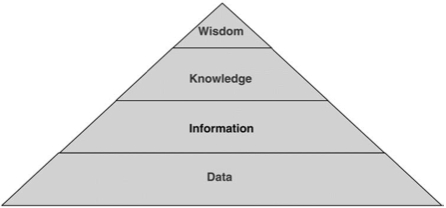
\includegraphics[height=1.5in]{knowledge-pyramid.png}
\end{center}

\begin{itemize}
\item Originally developed to describe the organization of knowledge
  in the mind
\item Higher levels are more abstract, require more processing to
  derive
\item Defines a lifecycle for data, which acquires meaning as it moves
  up the pyramid
\end{itemize}

\end{frame}
% --------------------------------------------------------------------------

% --------------------------------------------------------------------------
\begin{frame}{Data}

\begin{center}
\includegraphics[height=.5in]{data.png}
\end{center}

\begin{itemize}
\item Symbols or signals
\item Come directly from sensors
\end{itemize}

\end{frame}
% --------------------------------------------------------------------------

% --------------------------------------------------------------------------
\begin{frame}{Information}
\begin{center}
\includegraphics[height=.75in]{data-information.png}
\end{center}
\begin{itemize}
\item Information is data that have been transformed into a form that
  supports decision making or inference
\item Data are processed to produce information
\end{itemize}

\end{frame}
% --------------------------------------------------------------------------

% --------------------------------------------------------------------------
\begin{frame}{Knowledge and Wisdom}

\begin{center}
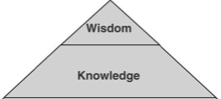
\includegraphics[height=1in]{knowledge-wisdom.png}
\end{center}

\begin{itemize}
\item Knowledge is typically ill-defined and often conflated with
  information, but loosely means information has been combined to
  provide context or reasoning.  Knowledge implies some understanding
  of the information
\item Can, to some extent, be mechanized in a computer system (this is
  what AI is all about).  For example, a spam filter automatically
  aquires knowledge about email to sort it
\end{itemize}
As information systems engineers, we leave (definitions of) knowledge
and wisdom to humans.

\end{frame}
% --------------------------------------------------------------------------

% --------------------------------------------------------------------------
\begin{frame}{DIKW in Information Systems}

Information systems engineers are concerned with turning data into
actionable information.  How?
\begin{itemize}
\item Structuring
\item Visualizing
\item Modeling
\end{itemize}
Once we turn data into information, humans can turn it into knowledge
and wisdom

\end{frame}
% --------------------------------------------------------------------------

% --------------------------------------------------------------------------
\begin{frame}{Structuring Data}

\begin{itemize}
\item Unstructured symbolic data, such as plain text, can be put into
  a logical structure in the mind by a human reader (and to some
  extent by AI systems)
\item Semi-structured symbolic data, such as XML or HTML documents, can be
  put into a logical structure for display or information exchange by
  automated information systems
\item Structured symbolic and quantitative data, such as a relational
  database, can support more complex queries on the data, such as
  ``how many papers did Stuart Russell publish in 2010?''
\end{itemize}

In this course, we'll learn how to structure data with XML and
relational databases.

\end{frame}
% --------------------------------------------------------------------------

% --------------------------------------------------------------------------
\begin{frame}{Visualizing Data}

Quantitative data can be plotted in a graphical display.  Information
can often be gleaned from these plots, such as:
\begin{columns}[t]
\begin{column}{2in}
\begin{center}
\includegraphics[width=1.4in]{beer.png}\\
\vspace{.1in}
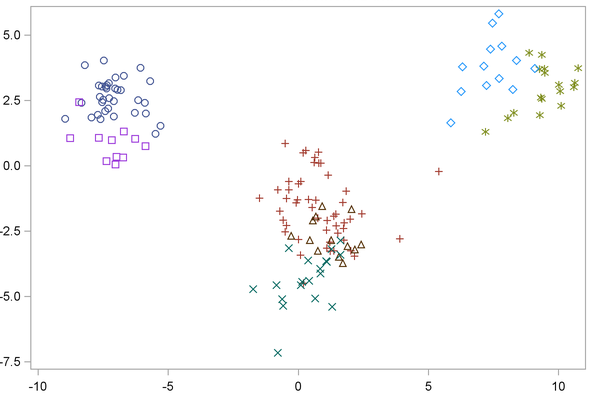
\includegraphics[width=1.3in]{clusters.png}
\end{center}
\end{column}
\begin{column}{2.5in}

\begin{itemize}
\item as one quantity increases, some other quantity increases, or
\vspace{.8in}
\item the data seem to cluster into distinct groups.
\end{itemize}
\end{column}
\end{columns}
\vspace{.1in}
In this course, we'll cover basic data visualization and delve into a
bit of Tufte's visual display wisdom.
\end{frame}
% --------------------------------------------------------------------------

% --------------------------------------------------------------------------
\begin{frame}{Modeling Data}

\begin{itemize}
\item Quantitative data can be modeled mathematically
\item A mathematical model has descriptive and predictive power
\item Mathematical models permit more precise inferences and
  decisions, such as
\begin{itemize}
\item inferring whether an improvement of a manufacturing process does
  or does not improve yield, or
\end{itemize}
\end{itemize}

In this course, we'll learn how to model data with basic ststistical
methods, emphasizing practical computational approaches rather than
theoretical understanding.

Note that some complex processes need to be modeled with simulation
techniques, which is the subject of ASE 6003 Modeling and Simulation.

\end{frame}
% --------------------------------------------------------------------------

% --------------------------------------------------------------------------
\begin{frame}{Information Systems Thinking}

Information systems are components of other systems -- think ``system
of systems''

\begin{itemize}
\item Data come from sensors
\begin{itemize}
\item I highly recommend looking at the materials for ASE 6111 Sensor Systems
\end{itemize}
\item Information is used by other systems, for example
\begin{itemize}
\item humans in the loop take decisions based on information
\item control systems use information to activate actuators
\end{itemize}
\end{itemize}

\end{frame}
% --------------------------------------------------------------------------

% --------------------------------------------------------------------------
\begin{frame}{Elements of Information Systems}

\begin{itemize}
\item Computers: we'll deal mostly with software, but we need to
  understand a little about the computers that run the software
\item Networks: computers are far more powerful and compelling when networked
\item Security: cannot be ignored.  You wouldn't leave your car
  unlocked in a bad neighborhood, and every internetworked computer
  lives in a bad neighborhood
\end{itemize}

\end{frame}
% --------------------------------------------------------------------------

% --------------------------------------------------------------------------
\begin{frame}{Information Systems Development}

Systems engineering is about lifecycles.  We've seen a sort of ``data
becomes information'' lifecycle.  We'll also learn the information
system development lifecycle, also called the software development
life cycle, which is highlighted by:
\begin{itemize}
\item requirements, where we determine exactly what our system is
  supposed to do;
\item design, where we determine the structure of the system that will
  meet our requirements;
\item implementation, where we build what we have designed;
\item testing, where we confirm that our system works according to
  specifications, and
\item deployment, where we put our system in the hands of its users
\end{itemize}

\end{frame}
% --------------------------------------------------------------------------

% --------------------------------------------------------------------------
\begin{frame}{Conclusion}

In this course we'll
\begin{itemize}
\item learn what information sytems are made of,
\item gain practical computational skills in turning data into
  information, and
\item learn how to develop information systems to meet specific
  customer needs.
\end{itemize}

\end{frame}
% --------------------------------------------------------------------------

%% % --------------------------------------------------------------------------
%% \begin{frame}{}

%% \begin{itemize}
%% \item
%% \end{itemize}

%% \end{frame}
%% % --------------------------------------------------------------------------

\end{document}
